% !TEX program = pdflatex
% CESG 2026 poster: The Blessings of Overparameterization
% Board: horizontal, 4ft x 8ft. Poster designed at 48in x 72in (landscape), centered on the board.
\documentclass[final]{beamer}
\usepackage[orientation=landscape,size=custom,width=182.88,height=121.92,scale=1.35]{beamerposter}

\usepackage{booktabs}
\usepackage{graphicx}
\usepackage{xcolor}
\usepackage{amssymb}
\usepackage{amsmath}
\usepackage{dsfont}
\usepackage[many]{tcolorbox}

\graphicspath{{figures/}}

% ---- colors from the deck ----
\definecolor{KahouBlack}{RGB}{31, 28, 26}
\definecolor{KahouGold}{RGB}{201, 168, 76}
\definecolor{KahouLightGold}{RGB}{240, 225, 180}
\definecolor{emphcolorval}{RGB}{128, 0, 32}
\definecolor{Terracotta}{RGB}{180, 90, 60}
\definecolor{TerracottaLight}{RGB}{242, 236, 220}
\definecolor{Sienna}{RGB}{120, 55, 25}
\definecolor{SlideBackground}{RGB}{252, 249, 240}

\setbeamercolor{background canvas}{bg=SlideBackground}
\setbeamercolor{block title}{fg=white, bg=Terracotta}
\setbeamercolor{block body}{fg=KahouBlack, bg=TerracottaLight}
\setbeamercolor{headline}{fg=KahouBlack, bg=SlideBackground}
\setbeamercolor{item}{fg=Terracotta}

\newcommand{\emphcolor}[1]{\textbf{\textcolor{emphcolorval}{#1}}}
\newcommand{\Xdom}{\mathcal{X}}
\newcommand{\F}{\mathcal{F}}
\newcommand{\R}{\mathcal{R}}

% block appearance
\setbeamertemplate{block begin}{
  \vskip.5ex
  \begin{beamercolorbox}[rounded=true,leftskip=1.2cm,colsep*=.75ex]{block title}
    \usebeamerfont{block title}\large\bfseries\insertblocktitle
  \end{beamercolorbox}
  \vskip-.3ex
  \usebeamerfont{block body}
  \begin{beamercolorbox}[rounded=true,colsep*=.75ex,vmode]{block body}
  \begin{minipage}{0.96\textwidth}\vskip1ex
}
\setbeamertemplate{block end}{\end{minipage}\vskip1ex\end{beamercolorbox}\vskip2ex}

\setbeamertemplate{itemize item}{\textcolor{Terracotta}{\textbf{--}}}
\setbeamertemplate{itemize subitem}{\textcolor{Sienna}{$\circ$}}
\setbeamertemplate{navigation symbols}{}

% a highlighted equation box
\newtcolorbox{eqbox}{enhanced, colback=KahouLightGold, colframe=KahouGold,
  boxrule=1pt, arc=4pt, left=6pt, right=6pt, top=4pt, bottom=4pt, halign=center}

\newlength{\sepwid}
\newlength{\onecolwid}
\setlength{\sepwid}{0.022\paperwidth}
\setlength{\onecolwid}{0.30\paperwidth}
\newlength{\colheight}
\setlength{\colheight}{3000pt}

\begin{document}
\begin{frame}[t]

% ================= HEADER =================
\begin{beamercolorbox}[wd=\paperwidth,sep=0pt]{headline}
\vskip0.3ex
\begin{columns}[c]
  \begin{column}{0.16\paperwidth}
    \centering
    {\color{KahouGold}\rule{0.8\textwidth}{6pt}}\\[0.5ex]
    {\large\textbf{CESG 2026}}\\[0.3ex]
    {\normalsize Vancouver}\\[0.5ex]
    {\color{KahouGold}\rule{0.8\textwidth}{6pt}}
  \end{column}
  \begin{column}{0.66\paperwidth}
    \centering
    {\veryHuge\textbf{\textcolor{KahouBlack}{The Blessings of Overparameterization}}}\\[1.0ex]
    {\Huge\textcolor{Sienna}{Applications in Solving Economic Models}}\\[1.2ex]
    {\Large Mahdi E. Kahou$^{1}$ \qquad Jes\'{u}s Fern\'{a}ndez-Villaverde$^{2}$}\\[0.6ex]
    {\large $^{1}$Bowdoin College \qquad $^{2}$University of Pennsylvania}
  \end{column}
  \begin{column}{0.16\paperwidth}
    \centering
    {\color{KahouGold}\rule{0.8\textwidth}{6pt}}\\[0.5ex]
    {\large\textbf{The moral}}\\[0.3ex]
    {\normalsize The parameter count\\ was never the risk.}\\[0.5ex]
    {\color{KahouGold}\rule{0.8\textwidth}{6pt}}
  \end{column}
\end{columns}
\vskip0.3ex
\end{beamercolorbox}
\vskip1ex
{\color{Terracotta}\rule{\paperwidth}{3pt}}
\vskip1ex

% ================= BODY: 3 COLUMNS =================
\begin{columns}[t]

% ---------- COLUMN 1: setup + question ----------
\begin{column}{\onecolwid}
\begin{minipage}[t][\colheight][s]{\linewidth}
\Large

\begin{block}{Motivation}
  Deep learning now solves \emphcolor{high-dimensional} dynamic models once thought intractable. But these networks are \emphcolor{massively overparameterized}: far more parameters than ``data'' points.
  \vskip1ex
  The classical worry is \emphcolor{overfitting} and poor out-of-grid performance. One key difference from statistics: our residuals are deterministic evaluations of the functional equation, so there is \emphcolor{no noise to overfit}. The question is what the algorithm does \emphcolor{between the grid points}.
\end{block}

\vfill

\begin{block}{The question}
  When we solve dynamic models with neural networks, is overparameterization a \emphcolor{necessary evil}, or does it buy us something?
\end{block}

\vfill

\begin{block}{Setup: models as functional equations}
  An economic object $f:\Xdom\to\R\subseteq\mathbb{R}^d$ (a policy, a value function) with model error $\ell(x,f)$ (Euler or Bellman residual). A \emphcolor{solution} satisfies $\ell(x,f^\star)=\mathbf{0}$ for all $x$.
  \vskip1ex
  Pick a parametric family $f(\cdot;\theta)$, sample a grid $\mathcal{D}=\{x_1,\dots,x_N\}$, and minimize the mean squared residual:
  \vskip1ex
  \begin{eqbox}
  $\displaystyle \min_{\theta}\ \mathcal{L}(\theta;\mathcal{D}) = \frac{1}{N}\sum_{x\in\mathcal{D}} \big\| \ell\big(x,f(\cdot;\theta)\big)\big\|_2^2$
  \end{eqbox}
  \vskip1ex
  Neural networks are a \emphcolor{highly overparameterized} class ($M\gg N$). Training is \emphcolor{non-convex}, so the solution can depend on the \emphcolor{initialization}. We run \emphcolor{50 seeds} at every width.
\end{block}

\vfill

\begin{block}{What we find}
  \begin{itemize}
    \item \emphcolor{Accuracy improves with size.} Wider networks give more accurate solutions.
    \item \emphcolor{Stability improves with size.} The spread across seeds collapses as width grows.
    \item \emphcolor{A mechanism.} In a dissectable random-features case: width buys agreement, the implicit bias decides what you agree on.
  \end{itemize}
\end{block}

\vfill

\begin{block}{Four models of increasing difficulty}
  \begin{itemize}
    \item \emphcolor{Linear-Quadratic:} closed form, sharpest test of error.
    \item \emphcolor{McCall job search:} 1D, kink at the reservation wage.
    \item \emphcolor{Real Business Cycle:} 2D stochastic state, no closed form, benchmarked vs.\ VFI.
    \item \emphcolor{Small Open Economy:} 5D, three shocks, beyond any grid benchmark.
  \end{itemize}
  \vskip0.5ex
  This poster details the first two and the random-features dissection. In all four, \emphcolor{accuracy} and \emphcolor{stability} improve with overparameterization.
\end{block}

\end{minipage}
\end{column}

% ---------- COLUMN 2: basic results ----------
\begin{column}{\onecolwid}
\begin{minipage}[t][\colheight][s]{\linewidth}
\large

\begin{block}{The two worked models}
  \emphcolor{Linear-Quadratic.} A price-taking firm chooses investment $u$ at quadratic adjustment cost, state $(y,Y)$:
  \vskip0.5ex
  \begin{eqbox}
  $\begin{array}{c}
  \displaystyle v(y,Y)=\max_{u}\ (\alpha_0-\alpha_1 Y)y-\tfrac{\gamma}{2}u^2+\beta\,v(y',Y')\\[1.2ex]
  \text{s.t.}\quad y'=y+u,\qquad Y'=h_0+h_1 Y
  \end{array}$
  \end{eqbox}
  \vskip1ex
  \emphcolor{McCall job search.} An unemployed worker gets i.i.d.\ offers $w\sim f$ on $[0,B]$ and accepts or keeps searching:
  \vskip0.5ex
  \begin{eqbox}
  $\displaystyle v(w)=\max\!\left\{\tfrac{w}{1-\beta},\ c+\beta\!\int_0^B v(w')f(w')\,dw'\right\}$
  \end{eqbox}
\end{block}

\vfill

\begin{block}{Result 1 -- Linear-Quadratic regulator}
  A competitive firm with quadratic adjustment costs. \emphcolor{Closed-form} solution, so the approximation error is known exactly at every point. Minimize the Euler residual over a grid of $n_Y=6$ points. Train and test loss stay \emphcolor{indistinguishable} at every width.
  \vskip1ex
  \centering
  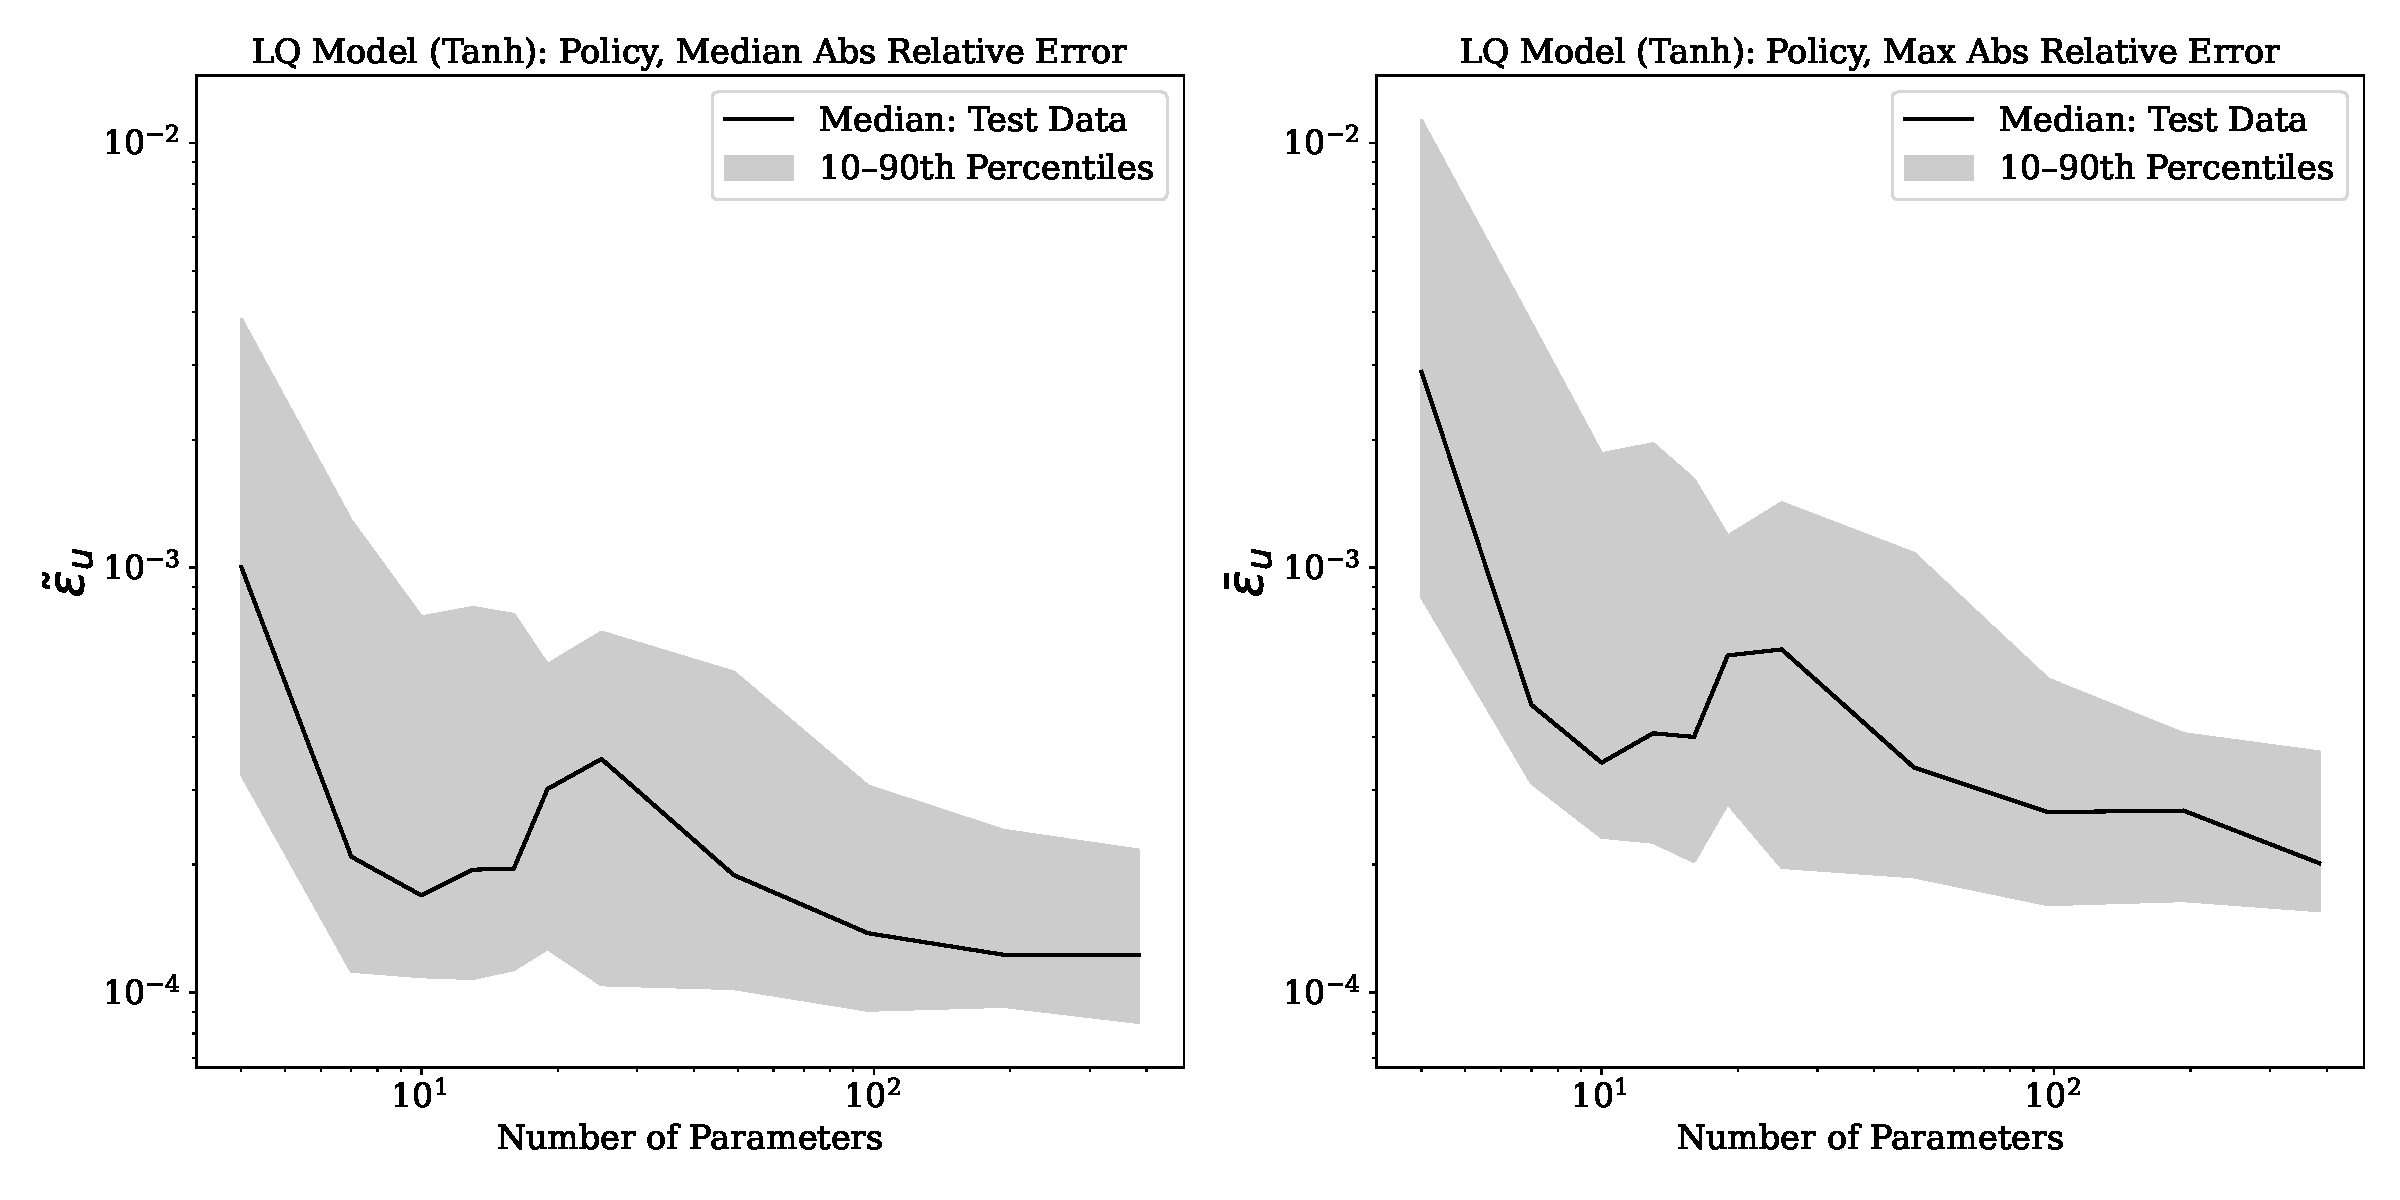
\includegraphics[width=0.95\textwidth]{LQ_policy_rel_error_median_vs_max_tanh}
  \vskip1ex
  \raggedright
  Median and max relative error fall to $\sim10^{-4}$ and the across-seed band narrows: accuracy \emphcolor{and} agreement improve together.
\end{block}

\vfill

\begin{block}{Result 2 -- McCall job search}
  Nonlinear and \emphcolor{non-smooth}: the value function has a \emphcolor{kink} at the reservation wage. The network must learn it from only $N=11$ points. Median relative error falls from $\sim17\%$ to $\sim0.2\%$, its plateau set by the kink, not the network.
  \vskip1ex
  \centering
  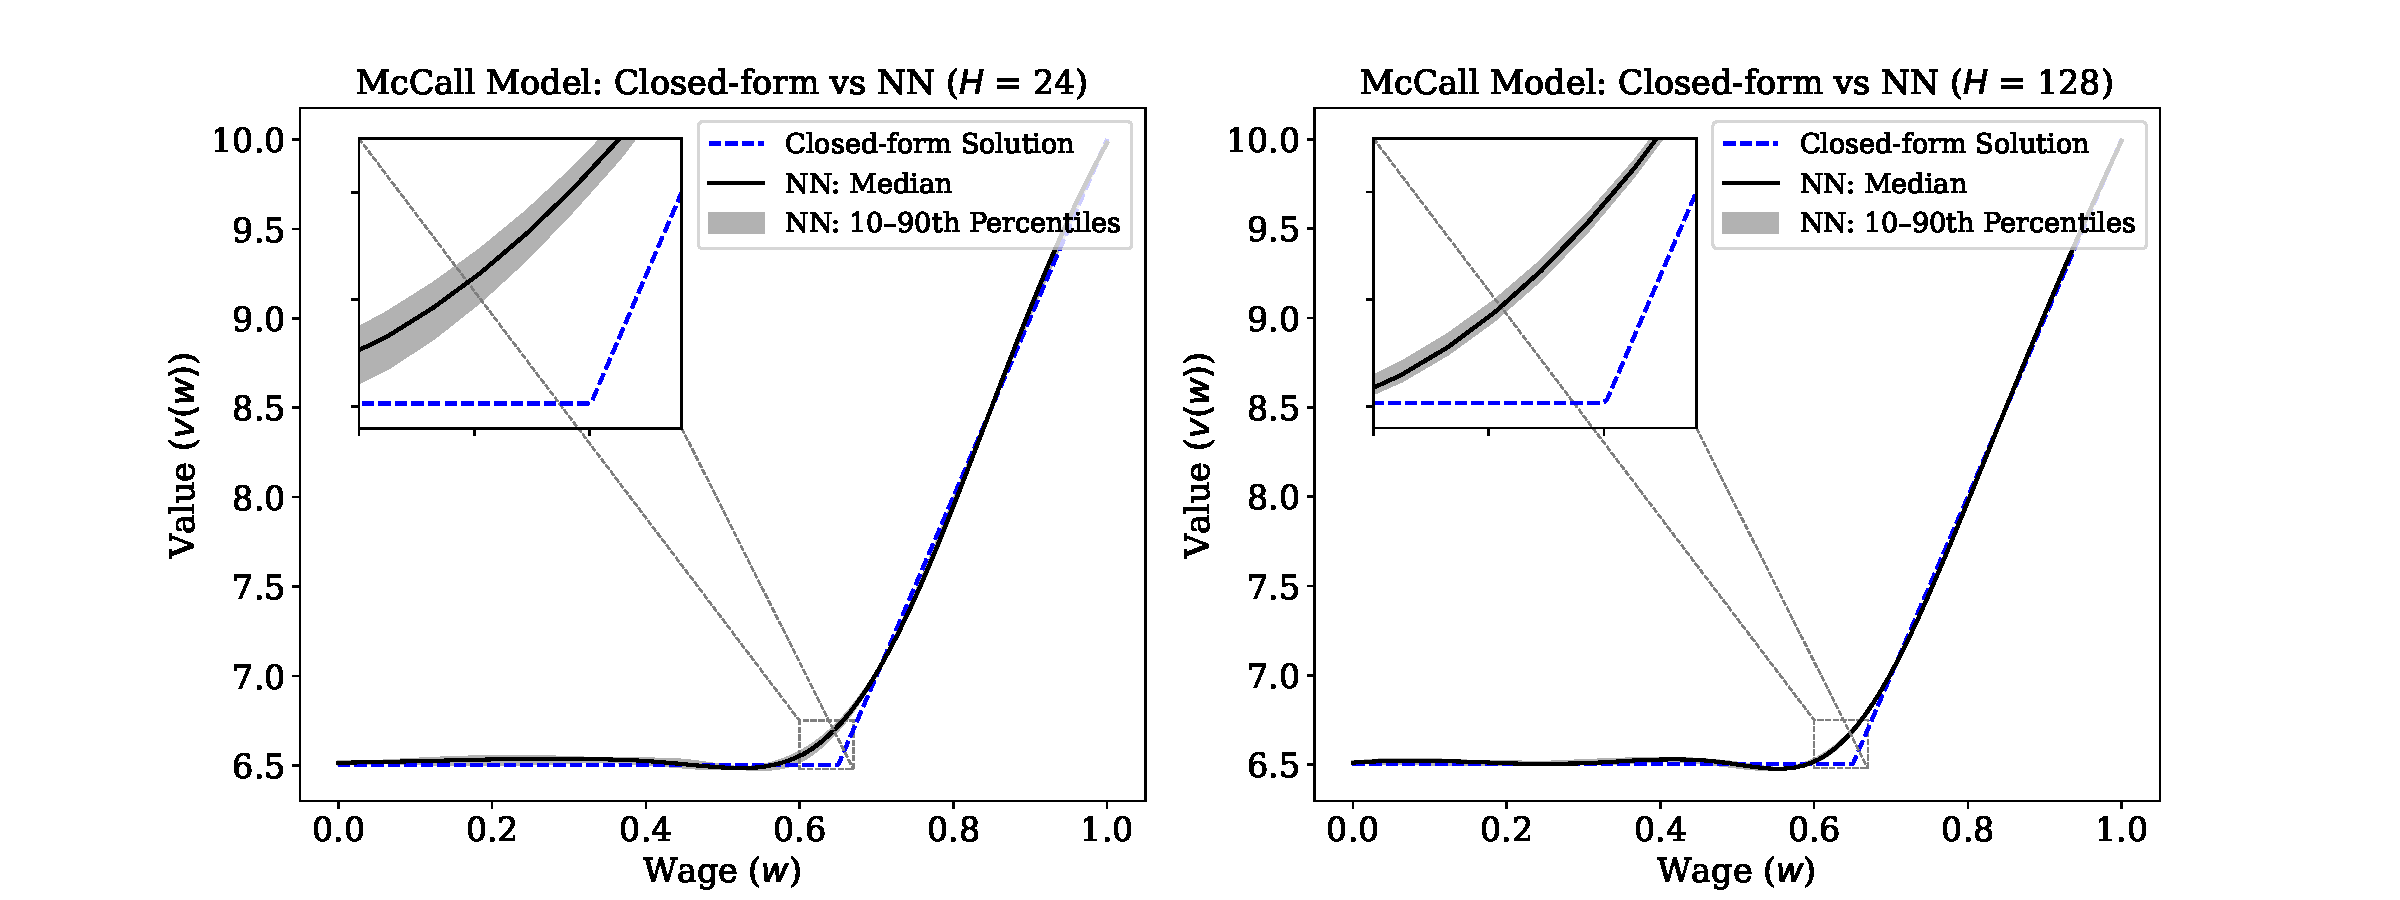
\includegraphics[width=0.95\textwidth]{McCall_value_function_24_vs_128_tanh}
  \vskip1ex
  \raggedright
  Narrow ($H=24$, left): the median tracks the truth but seeds disagree near the kink. Wide ($H=128$, right): 50 initializations \emphcolor{converge to the same function}, corner gently rounded. \emphcolor{Stability blessing confirmed.}
\end{block}

\end{minipage}
\end{column}

% ---------- COLUMN 3: careful examination ----------
\begin{column}{\onecolwid}
\begin{minipage}[t][\colheight][s]{\linewidth}

\begin{block}{A careful examination: random features}
  Something selects one solution among many. To see what, strip the model to a case where nothing is hidden: draw the first layer $(\tilde{w}_j,\tilde{b}_j)$ once, \emphcolor{freeze it}, train only the readout $\theta=(v_1,\dots,v_H,c)$:
  \vskip1ex
  \begin{eqbox}
  $\displaystyle f_H(Y;\theta) = \sum_{j=1}^{H} v_j\,\sigma(\tilde{w}_j Y + \tilde{b}_j) + c$
  \end{eqbox}
  \vskip1ex
  The LQ residual is then \emphcolor{linear in $\theta$}:
  \vskip1ex
  \begin{eqbox}
  $\displaystyle \Phi\,\theta = d, \qquad \Phi\in\mathbb{R}^{N\times(H+1)}$
  \end{eqbox}
  \vskip1ex
  For $H+1>N$ there are \emphcolor{infinitely many exact solutions}. The loss cannot identify $\theta$: \emphcolor{the algorithm is the identifying assumption}. Gradient descent from zero converges to the minimum-norm interpolant
  \vskip1ex
  \begin{eqbox}
  $\displaystyle \theta^\star = \operatorname*{argmin}_{\theta:\,\Phi\theta=d}\ \|\theta\|_2 = \Phi^\top(\Phi\Phi^\top)^{-1}d$
  \end{eqbox}
  \vskip1ex
  which we solve directly, \emphcolor{bypassing training entirely}.
\end{block}

\vfill

\begin{block}{Minimum norm knows no economic model}
  \begin{columns}[t]
    \begin{column}{0.49\textwidth}\centering
      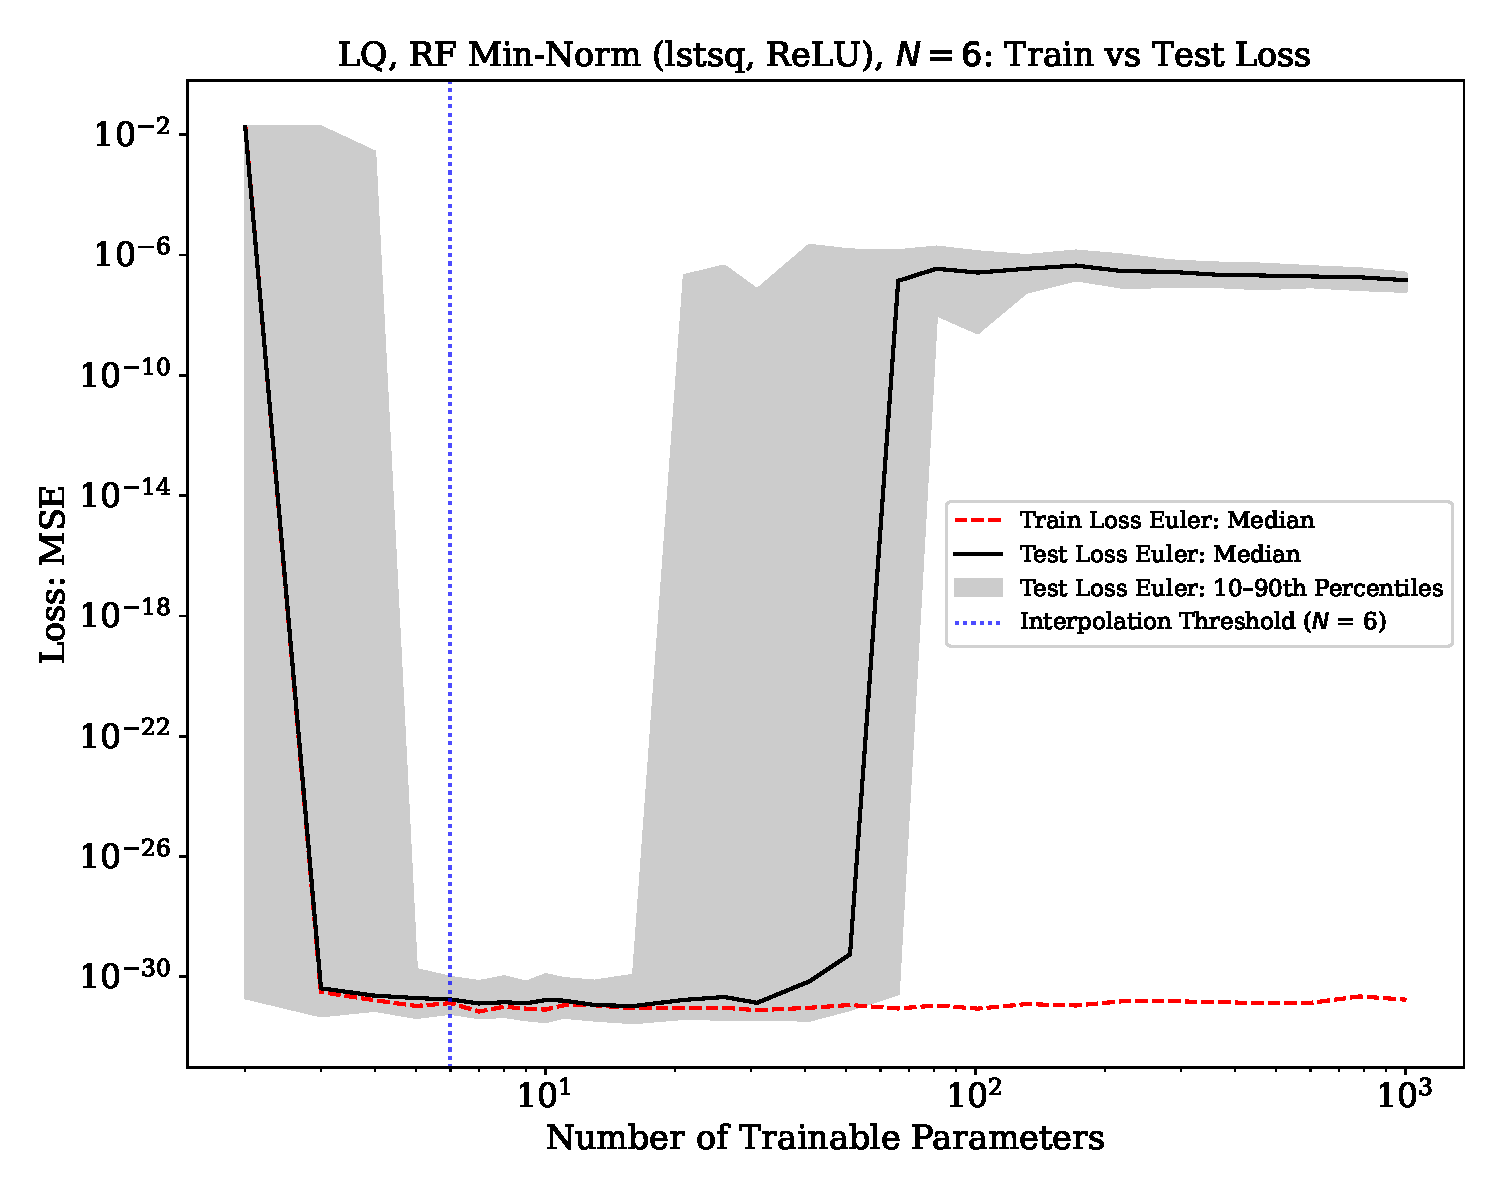
\includegraphics[width=\textwidth]{LQ_policy_RF_lstsq_N6_relu_test_train_loss}
    \end{column}
    \begin{column}{0.49\textwidth}\centering
      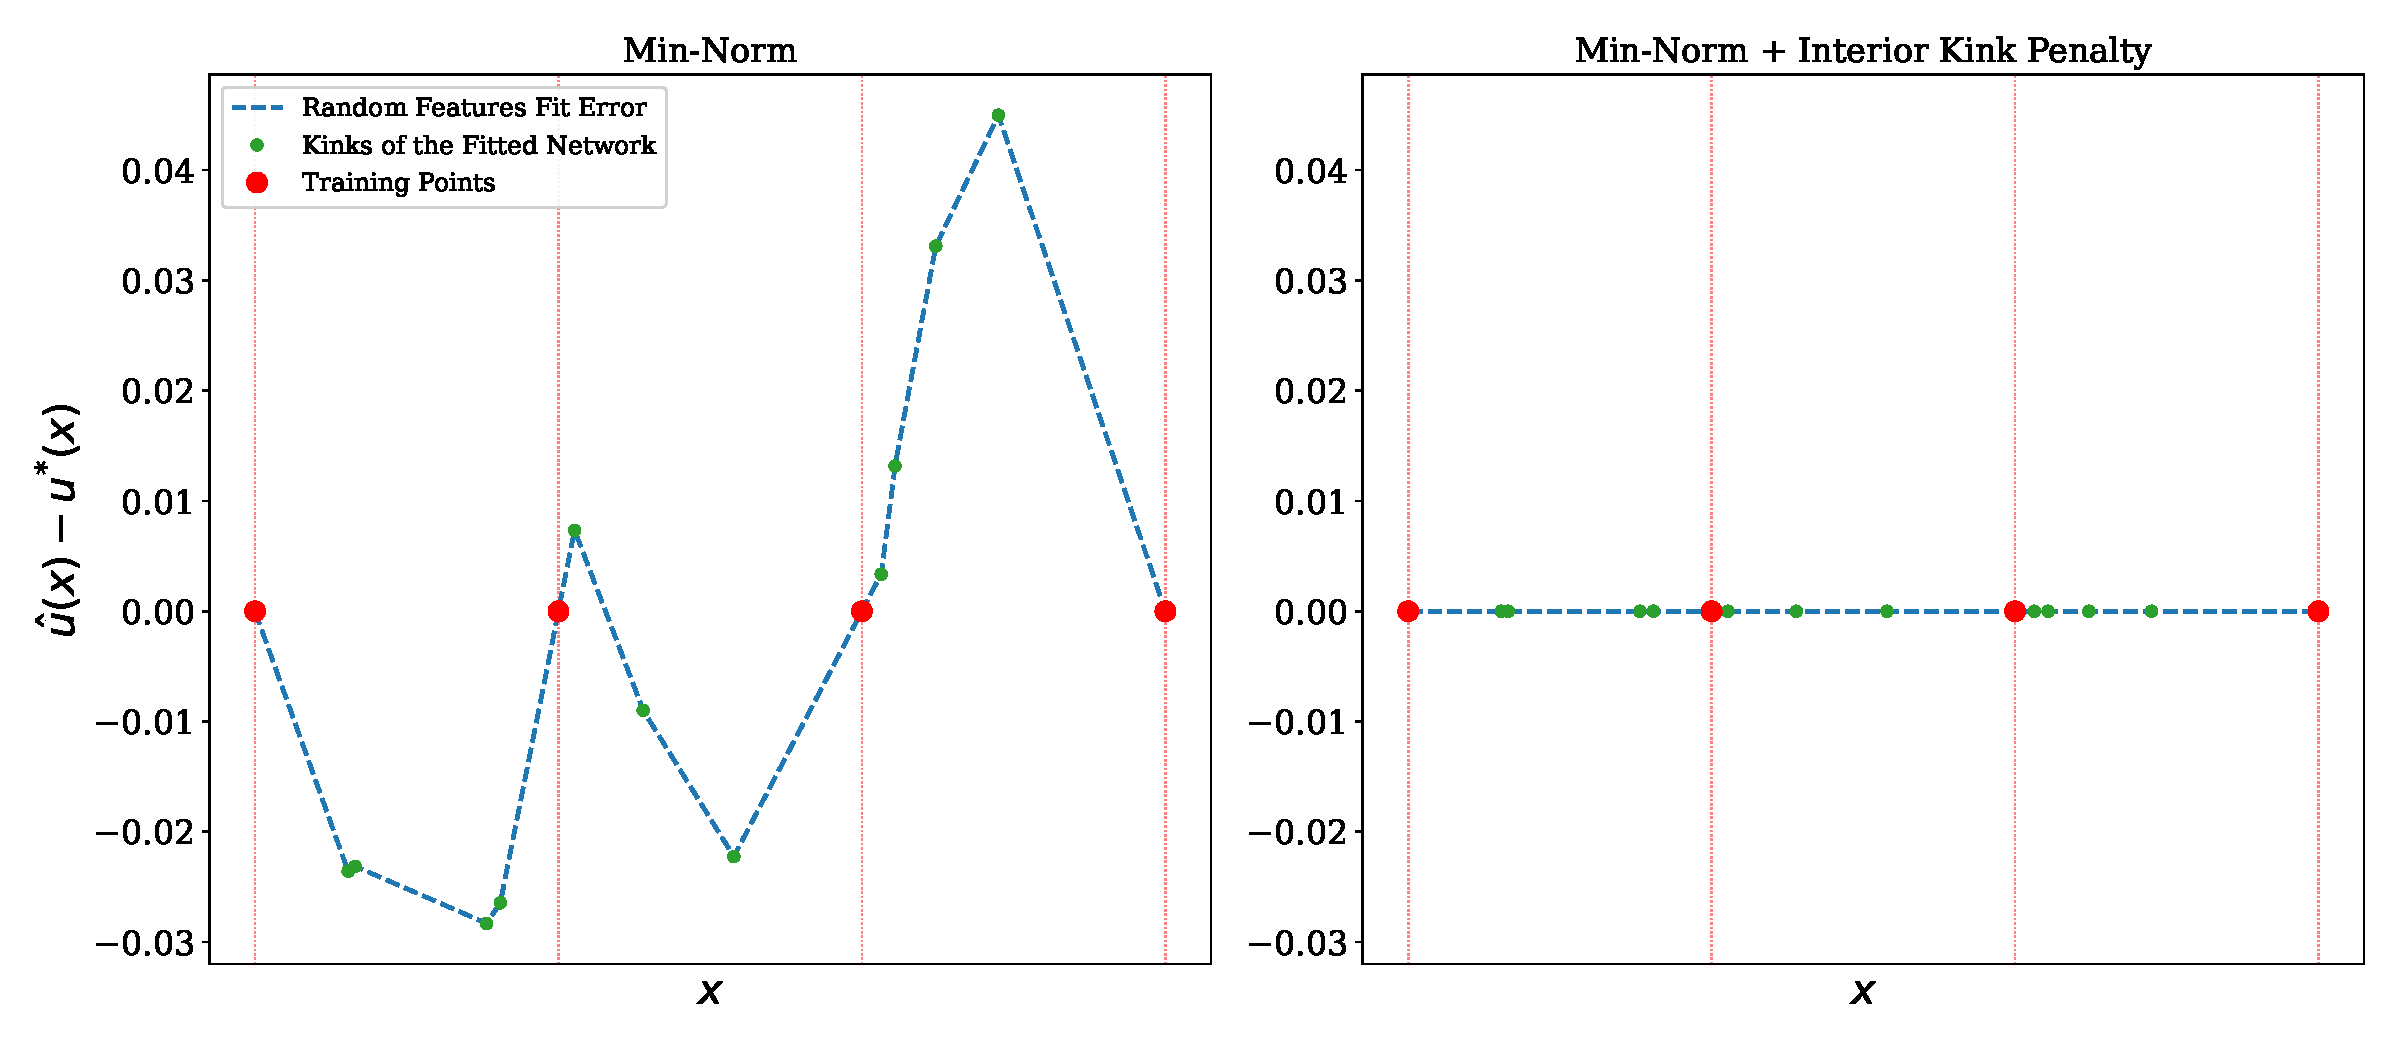
\includegraphics[width=\textwidth]{relu_bumps_illustration}
    \end{column}
  \end{columns}
  \vskip1ex
  With \emphcolor{ReLU} features the train loss is pinned at machine zero, but the test error \emphcolor{rises} with width. Min-norm in \emphcolor{coefficients} is not smoothness in \emphcolor{functions}: kinked features inject curvature between grid points, where the truth is linear. That is where the error lives.
\end{block}

\vfill

\begin{block}{The cure: penalize the kinks between points}
  \centering
  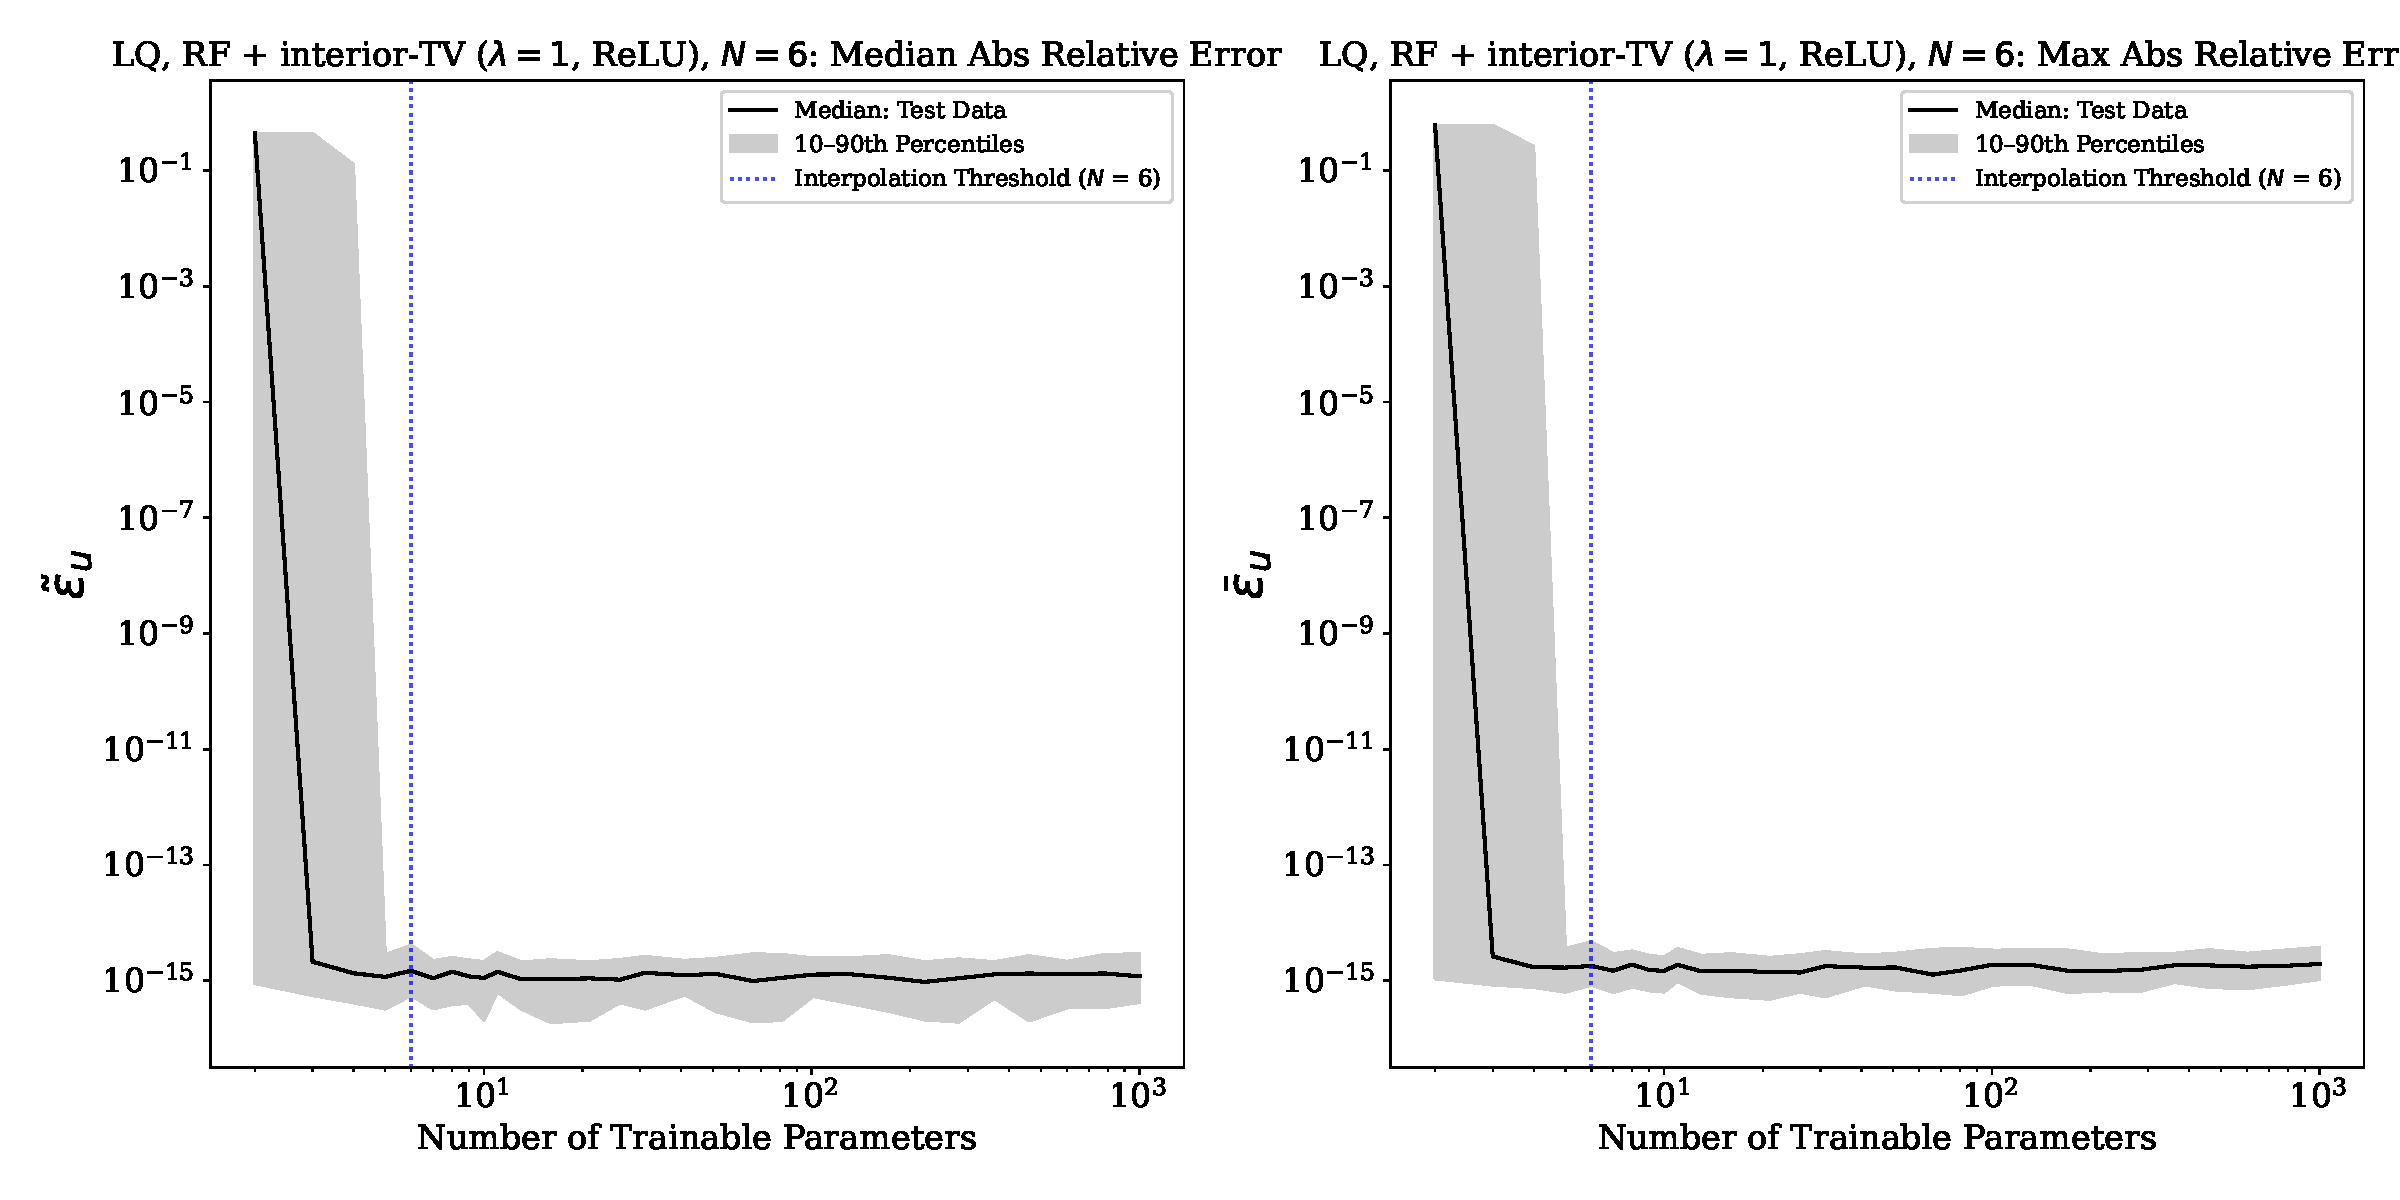
\includegraphics[width=0.74\textwidth]{LQ_policy_RF_lstsq_penalty_N6_relu_rel_error_median_vs_max}
  \vskip1ex
  \raggedright
  Charging for slope jumps inside the training range (a measure of interior curvature) snaps the fit back to the line: flat at $10^{-15}$ at every width.
\end{block}

\vfill

\begin{block}{Conclusion}
  Across four models (LQ, McCall, RBC, and a five-dimensional small open economy) and smooth activations, \emphcolor{out-of-sample residuals fall and seeds concentrate as width grows}. The mechanism: \emphcolor{width buys agreement; the implicit bias decides what you agree on}. The parameter count was never the risk.
\end{block}

\end{minipage}
\end{column}

\end{columns}

\end{frame}
\end{document}
